%\documentclass[handout]{beamer}
\documentclass[]{beamer}
%\usepackage[dvips]{color}
\usepackage{graphicx}
\usepackage{amsmath,amssymb,array,comment,eucal,url}
\input{../macros}
\usepackage{verbatim}

\usetheme{Warsaw}
\usecolortheme{orchid}
\title{Horseshoe, Lasso and Related Shrinkage Methods}
\subtitle{Readings Chapter 15 Christensen}
\institute{Merlise Clyde}
\author{STA721 Linear Models Duke University}
\date{\today}
\logo{duke.eps}

\begin{document}
\maketitle
\begin{frame}
  \frametitle{Bayesian Lasso}
  Park \& Casella (JASA 2008) and Hans (Biometrika 2010) propose
  Bayesian versions of the Lasso  \pause
  \begin{eqnarray*}
    \Y \mid \alpha, \b^s, \phi & \sim & \N(\one_n \alpha + \X^s \b^s, \I_n/\phi)  \pause\\
    \b^s \mid \alpha, \phi, \taub, \lambda & \sim & \N(\zero, \diag(\taub^2)/\phi)  \pause\\
    \tau_1^2 \ldots, \tau_p^2 \mid \alpha, \phi, \lambda & \simiid & \Ex(\lambda^2/2)  \pause\\
    p(\alpha, \phi) & \propto& 1/\phi  \pause\\
  \end{eqnarray*}
Can show that $\beta_j \mid \phi, \lambda \simiid DE(\lambda \sqrt{\phi})$
$$\int_0^\infty \frac{1}{\sqrt{2 \pi s}}
  e^{-\frac{1}{2} \phi \frac{\beta^2}{s }}
  \, \frac{\lambda^2}{2} e^{- \frac{\lambda^2 s}{2}}\, ds =
  \frac{\lambda \phi^{1/2}}{2} e^{-\lambda \phi^{1/2} |\beta|}
$$  \pause
Scale Mixture of Normals  (Andrews and Mallows 1974)
\end{frame}



\begin{frame}
  \frametitle{Gibbs Sampling}

Prior  $\lambda^2 \sim \Gam(r,\delta)$ \pause  Integrate out $\alpha$: $\alpha \mid \Y, \phi \sim \N(\ybar,     1/(n \phi)$  \pause

Full Conditionals
  \begin{itemize}
 \item $\b^s \mid \taub, \phi, \lambda, \Y \sim \N(, )$   \pause
\item $\phi \mid \taub, \b^s, \lambda, \Y \sim \G( , ) $  \pause
\item $\lambda^2\mid  \b^s, \phi, \tau^2, \Y \sim \G( , )$ \pause
\item $1/\tau_j^2 \mid \b^s, \phi, \lambda, \Y \sim \text{InvGaussian}(
  , )$  \pause
 \end{itemize}
$X \sim \textsf{InvGaussian}(\mu,  \lambda)$

$$
f(x) =  \sqrt{\frac{\lambda^2}{2 \pi}}  x^{-3/2} e^{- \frac{1}{2} \frac{
    \lambda^2( x - \mu)^2} {\mu^2 x}} \qquad x > 0
$$  \pause

Homework Nextweek:  Derive the full conditionals for $\b^s$, $\phi$,
$1/\tau^2$  see \url{http://www.stat.ufl.edu/~casella/Papers/Lasso.pdf} 
\end{frame}



\begin{frame}
  \frametitle{Horseshoe}
  Carvalho, Polson \& Scott  propose
\begin{itemize}
\item 
Prior Distribution on $$\b^s \mid \phi, \taub \sim \N(\zero_p, \frac{\diag(\taub^2)}{ \phi
    }) $$ \pause
\item $\tau_j \mid \lambda \simiid \C^+(0, \lambda^2)$   (difference is CPS notation) \pause
\item $\lambda \sim \C^+(0, 1)$ \pause
\item $p(\alpha, \phi) \propto 1/\phi)$ \pause
\end{itemize}

In the case $\lambda = \phi = 1$ and with canonical representation $\Y =
\I \b + \eps$ \pause
$$ 
E[\beta_i \mid \Y] = \int_0^1 (1 - \kappa_i) y^*_i p(\kappa_i \mid \Y)
\ d\kappa_i = (1 - \E[\kappa \mid y^*_i]) y^*_i$$
where $\kappa_i = 1/(1 + \tau_i^2)$ shrinkage factor \pause

\vspace{18pt}
Half-Cauchy prior induces a Beta(1/2, 1/2) distribution on $\kappa_i$
a priori
\end{frame}
\begin{frame}
\frametitle{Horseshoe}
  \includegraphics[height=3.5in]{beta}
\end{frame}

\begin{frame}
\frametitle{Prior Comparison (from PSC)}
  \includegraphics[height=3.5in]{densities}
\end{frame}

\begin{frame}
  \frametitle{Bounded Influence}
Normal means case      $Y_i \simiid N(\beta_i, 1)$    (Equivalent to Canonical case)
    \begin{columns}
    \begin{column}{.48\textwidth}
      \begin{itemize}
      \item 
Posterior mean
$E[\beta \mid y] = y + \frac{d} {d y} \log m(y)$
where $m(y)$ is the predictive denisty under the prior (known $\lambda$) \pause
\item HS has Bounded Influence: $$\lim_{|y| \to \infty} \frac{d}{dy} \log m(y) = 0$$ \pause
\item $\lim_{|y| \to \infty} E[\beta \mid y) \to y $ (MLE)\pause
\item DE is also bounded influence, but bound does not decay to zero in tails
      \end{itemize}

    \end{column}
    \begin{column}{.48\textwidth}
   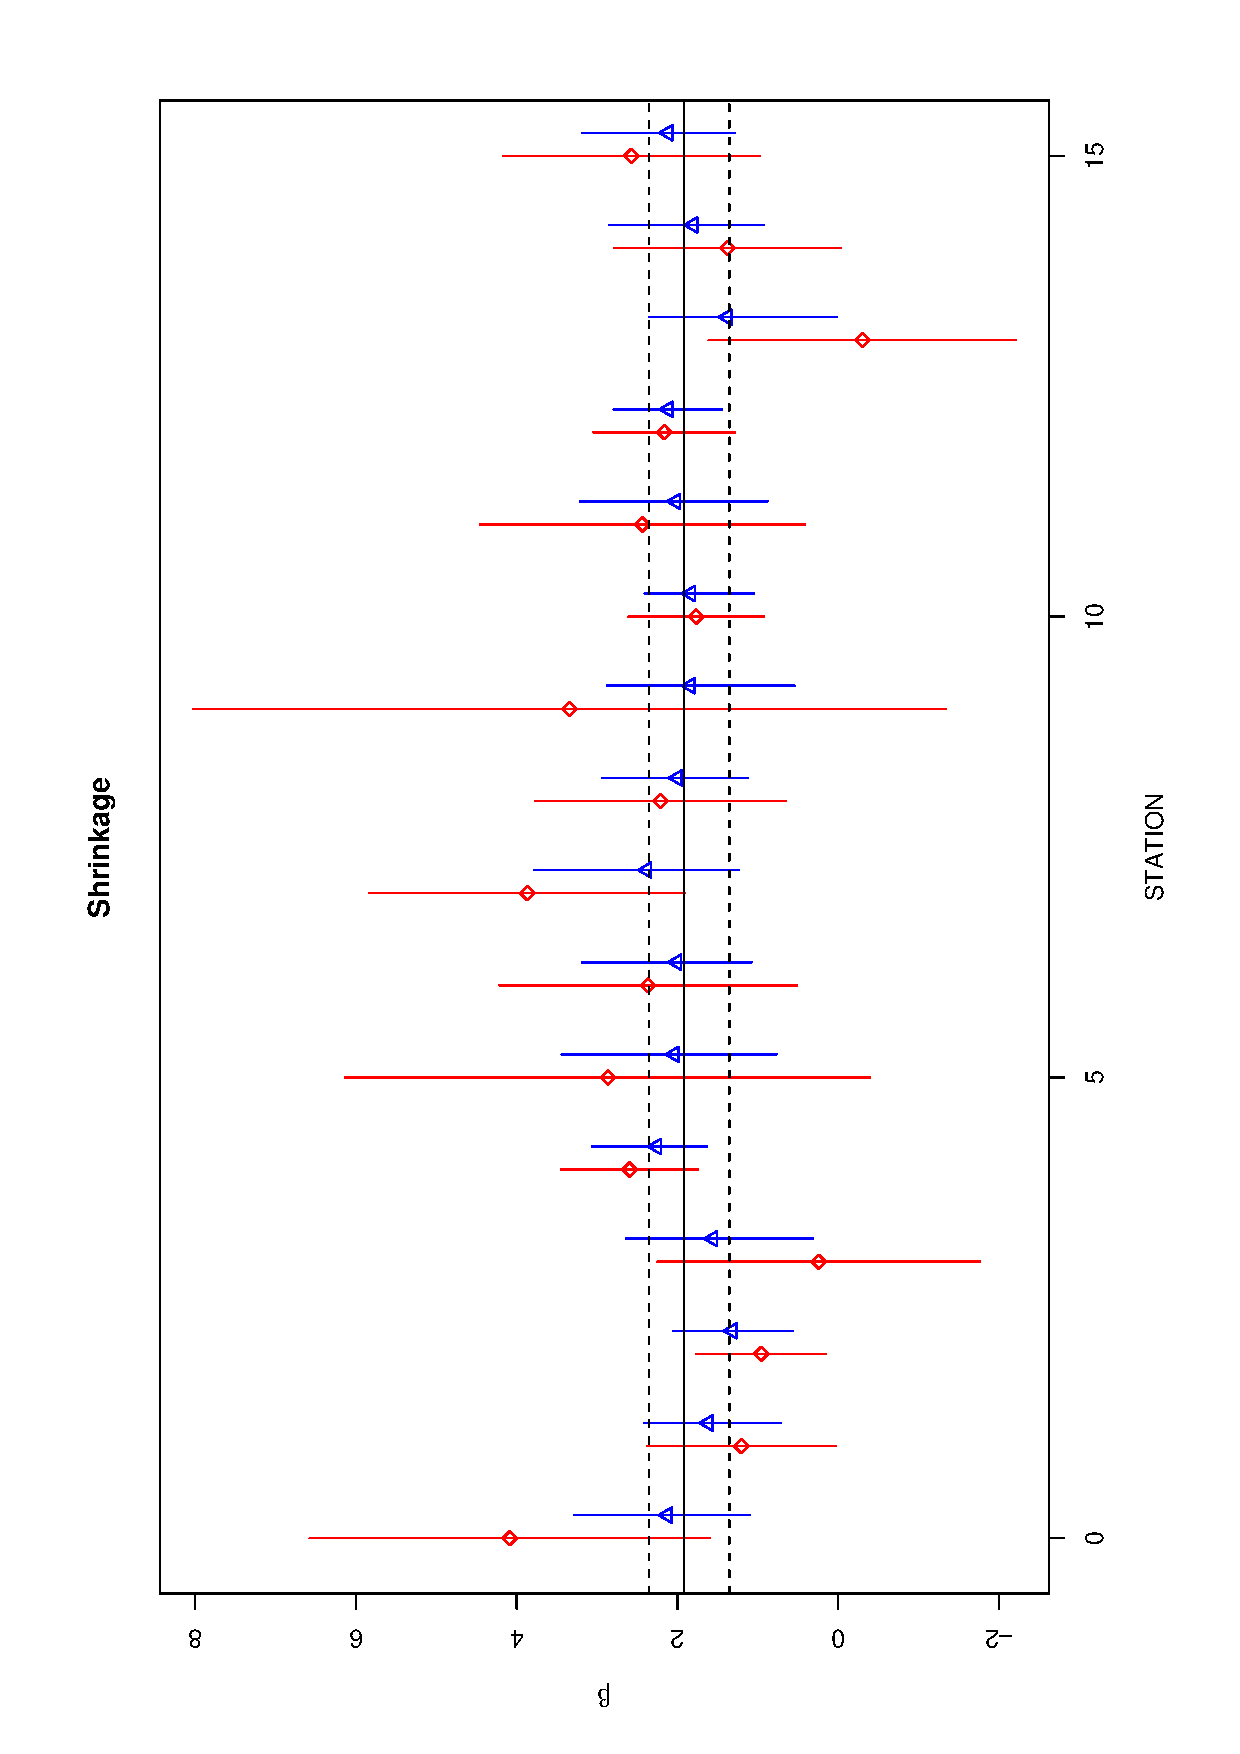
\includegraphics[width=2in]{shrinkage}
    \end{column}
      
    \end{columns}
\end{frame}

\begin{frame}
  \frametitle{R packages}
  The {\tt monomvn} package in R includes
  \begin{itemize}
  \item blasso
  \item bhs
  \end{itemize}

See Diabetes.R code 


  
\end{frame}

\begin{frame}
  \frametitle{Simulation Study with Diabetes Data}
  \includegraphics[height=3.5in]{diabetes}
 
  
\end{frame}

\begin{frame}
  \frametitle{Other Options}
  Range of other scale mixtures used  \pause
  \begin{itemize}
  \item Generalized Double Pareto (Armagan, Dunson \& Lee)  \pause
$\lambda \sim \Gam(\alpha, \eta)$  then $\beta^s_j \sim \textsf{GDP}(\xi
= \eta/\alpha, \alpha)$  \pause
$$
f(\beta^s_j) = \frac{1}{2 \xi} (1 + \frac{|\beta^s_j|}{\xi \alpha})^{-(1 + \alpha)}
$$

see \url{http://arxiv.org/pdf/1104.0861.pdf} \pause
  \item Normal-Exponenetial-Gamma (Griffen \& Brown 2005)
$\lambda^2 \sim \Gam(\alpha, \eta)$ 
  \pause
  \item Bridge - Power Exponential Priors  (Stable mixing density) \pause

   \end{itemize}
See the monomvn package on CRAN \pause

\vfill

Choice of prior?   Properties?  Fan \& Li (JASA 2001) discuss Variable
selection via nonconcave penalties and oracle properties
\end{frame}

\begin{frame}
  \frametitle{Choice of Estimator \& Selection?}

  \begin{itemize}
  \item Posterior Mode (may set some coefficients to zero) \pause
  \item Posterior Mean (no selection, just shrinkage) \pause
  \end{itemize}
  Bayesian Posterior does not assign any probability to $\beta^s_j = 0$ \pause

  \begin{itemize}
  \item selection based on posterior mode ad hoc rule - Select if
    $\kappa_i < .5)$ \pause \\
See  article by  Datta \& Ghosh
\url{http://ba.stat.cmu.edu/journal/forthcoming/datta.pdf} \pause
  \item Selection solved as a post-analysis decision problem \pause
  \item Selection part of model uncertainty $\Rightarrow$ add prior \pause
    probability that $\beta^s_j = 0$  and combine with decision problem 
  \end{itemize}
Remember all models are wrong, but some may be useful!
\end{frame}


\end{document}

